% 2011 年四川卷文科第 4 题：四个选项的函数图象（选项图）。
% 来源 PDF：普通高考/2011/2011四川文.pdf，SHA-256 9df4a6b69bb06bfab2f7d7ee0e7fcc50ae547f226260996d7a060c31ad14e64a。
% 原页：第 1 页（A3 三栏）第 1 栏中部，书页码 703。
% 重绘依据：照原页——(A) 递减、竖直渐近线 x=1、过 (2,0)，y 轴标 1、x 轴标 1 与 2；
%   (B) 递增、竖直渐近线 x=1、过 (2,0)，y 轴标 1、x 轴标 1 与 2；
%   (C) 递增、过 (0,2)、水平渐近线 y=1，y 轴标 2（曲线与 y 轴交点处）与 1，x 轴标 1；
%   (D) 递增、与 x 轴交点处标 −2、x 轴另标 −1、y 轴标 1，左端渐平（渐近线在 x 轴下方）。
%   四个选项各为独立的直角坐标系，(A)(B) 在上行、(C)(D) 在下行，字母在各自图形左下，照原页。
%   说明：(D) 只是干扰项，原页未给函数式，仅按可辨认的拓扑（增、下凸、在负半轴穿过 x 轴、
%   y 轴截距 1、左端有水平渐近线）重绘，取 y=2^{x/2+1}-1 作图，不按原页比例，不代表某个确定函数。
%   原页各图均无网格、无虚线。
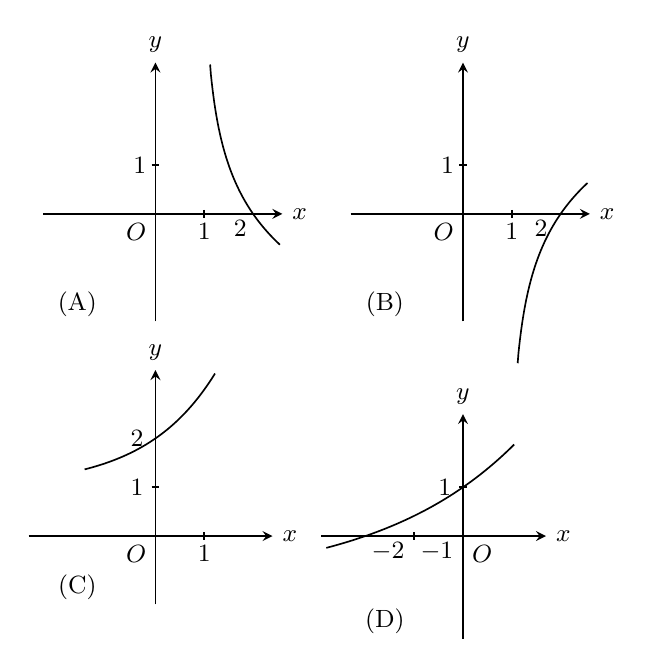
\begin{tikzpicture}[scale=0.62, >=stealth, semithick, font=\small]

  % ================= (A) =================
  \begin{scope}
    \draw[->] (-2.3,0) -- (2.6,0) node[right] {$x$};
    \draw[->] (0,-2.2) -- (0,3.1) node[above] {$y$};
    \draw (1,0.08) -- (1,-0.08);
    \draw (-0.08,1) -- (0.08,1);
    \node[below left, inner sep=3pt] at (0,0) {$O$};
    \node[below, inner sep=3pt] at (1,0) {$1$};
    \node[below left, inner sep=2pt] at (2,0) {$2$};
    \node[left, inner sep=3pt] at (0,1) {$1$};
    \draw[domain=1.12:2.55, samples=90] plot (\x,{-ln(\x-1)/ln(2)});
    \node at (-1.6,-1.85) {(A)};
  \end{scope}

  % ================= (B) =================
  \begin{scope}[shift={(6.3,0)}]
    \draw[->] (-2.3,0) -- (2.6,0) node[right] {$x$};
    \draw[->] (0,-2.2) -- (0,3.1) node[above] {$y$};
    \draw (1,0.08) -- (1,-0.08);
    \draw (-0.08,1) -- (0.08,1);
    \node[below left, inner sep=3pt] at (0,0) {$O$};
    \node[below, inner sep=3pt] at (1,0) {$1$};
    \node at (1.60,-0.30) {$2$};
    \node[left, inner sep=3pt] at (0,1) {$1$};
    \draw[domain=1.12:2.55, samples=90] plot (\x,{ln(\x-1)/ln(2)});
    \node at (-1.6,-1.85) {(B)};
  \end{scope}

  % ================= (C) =================
  \begin{scope}[shift={(0,-6.6)}]
    \draw[->] (-2.6,0) -- (2.4,0) node[right] {$x$};
    \draw[->] (0,-1.4) -- (0,3.4) node[above] {$y$};
    \draw (1,0.08) -- (1,-0.08);
    \draw (-0.08,1) -- (0.08,1);
    \node[below left, inner sep=3pt] at (0,0) {$O$};
    \node[below, inner sep=3pt] at (1,0) {$1$};
    \node[left, inner sep=4pt] at (0,1) {$1$};
    \node[left, inner sep=4pt] at (0,2) {$2$};
    \draw[domain=-1.45:1.22, samples=90] plot (\x,{exp(\x*ln(2))+1});
    \node at (-1.6,-1.05) {(C)};
  \end{scope}

  % ================= (D) =================
  \begin{scope}[shift={(6.3,-6.6)}]
    \draw[->] (-2.9,0) -- (1.7,0) node[right] {$x$};
    \draw[->] (0,-2.1) -- (0,2.5) node[above] {$y$};
    \draw (-1,0.08) -- (-1,-0.08);
    \draw (-0.08,1) -- (0.08,1);
    \node[below right, inner sep=3pt] at (0,0) {$O$};
    \node[below right, inner sep=2pt] at (-2,0) {$-2$};
    \node[below right, inner sep=2pt] at (-1,0) {$-1$};
    \node[left, inner sep=4pt] at (0,1) {$1$};
    \draw[domain=-2.8:1.05, samples=90] plot (\x,{exp((\x/2+1)*ln(2))-1});
    \node at (-1.6,-1.75) {(D)};
  \end{scope}

\end{tikzpicture}
